\section{矩阵分析}
\subsection{矩阵序列与矩阵级数}
\subsubsection{矩阵序列及收敛性}
设$\{A^{(k)}\},k=1,2,\cdots,$是$C^{m\times n}$矩阵序列,$A^{(k)}=(a_{ij})_{m\times n},\|\cdot\|$是$C^{m\times n}$上任一矩阵范数,矩阵序列$\{A^{(k)}\}$收敛于$A$,有
\[
\begin{split}
 \colorbox{yellow}{$\lim\limits_{k\rightarrow \infty}A^{(k)}=A$} &\colorbox{yellow}{$\Leftrightarrow	\lim\limits_{k\rightarrow \infty}a_{ij}^{(k)}=a_{ij}$}\quad(1\leq i \leq m,1<j<n)   \\
	&\Leftrightarrow	\lim\limits_{k\rightarrow \infty}|a_{ij}^{(k)}-a_{ij}|=0\quad(1\leq i \leq m,1<j<n)\\
	&\colorbox{yellow}{$\Leftrightarrow	\lim\limits_{k\rightarrow \infty}\|A^{(k)}-A\|=0 $}
 \end{split}
\]

\noindent 矩阵序列满足的性质:
\begin{theorem}

	设$\lim\limits_{k\rightarrow \infty}A^{(k)}=A,\lim\limits_{k\rightarrow \infty}B^{(k)}=B,\alpha ,\beta\in C$,则
	\begin{enumerate}
		\item \colorbox{yellow}{$\lim\limits_{k\rightarrow \infty}(\alpha A^{(k)} +\beta B^{(k)})=\alpha A +\beta B$ }
		\item\colorbox{yellow}{$\lim\limits_{k\rightarrow \infty}(A^{(k)} B^{(k)})= AB$ }
		\item 当$A^{(k)}$和$A$都可逆时,\colorbox{yellow}{$\lim\limits_{k\rightarrow \infty}(A^{(k)})^{-1} = A^{-1}$}
	\end{enumerate}
\end{theorem}
\textcolor{red}{方阵的幂构成的矩阵序列(重要)}
\begin{theorem}
	\label{hhvcf}
\colorbox{yellow}{设$A\in C^{n\times n}$,则$\lim\limits_{k\rightarrow \infty}A^k=0\mbox{($A$为收敛矩阵)}\Leftrightarrow r(A)<1 \Leftrightarrow $存在\textcolor{red}{相容矩阵范数}$\|A\|_m<1$}
\end{theorem}
\subsubsection{矩阵级数及收敛性}
设$\{A^{(k)}\},k=1,2,\cdots,$是$C^{m\times n}$矩阵序列,则称\colorbox{yellow}{$\sum\limits_{k=1}^{\infty}A^{(k)}$}为矩阵级数,称\colorbox{yellow}{$S^N=\sum\limits_{k=1}^{N}A^{(k)}$}为矩阵级数的部分和.
\[
\begin{split}
&\colorbox{yellow}{$\sum\limits_{k=1}^{\infty}A^{(k)}$收敛($\lim\limits_{N\rightarrow \infty}S^N=S) \Leftrightarrow \lim\limits_{N\rightarrow \infty}s_{ij}^N=\lim\limits_{N\rightarrow \infty}\sum\limits_{k=1}^{N}a_{ij}^{(k)}=s_{ij}(i=1,2,\cdots,m;j=1,2,\cdots,n)$}\\
&\colorbox{yellow}{$\Leftrightarrow\sum\limits_{k=1}^{\infty}a_{ij}^{(k)}(i=1,2,\cdots,m;j=1,2,\cdots,n)$\mbox{收敛} $\Rightarrow \lim\limits_{k\rightarrow \infty}a_{ij}^{(k)}=0 \Rightarrow \lim\limits_{k\rightarrow \infty}A^{(k)}=0$}
\end{split}
\]

此外,有:
\[
\begin{split}
	&\colorbox{yellow}{$ \sum\limits_{k=1}^{\infty}A^{(k)}\mbox{绝对收敛} \Leftrightarrow \sum\limits_{k=1}^{\infty}|a_{ij}^{(k)}|\mbox{收敛}\Rightarrow \sum\limits_{k=1}^{\infty}a_{ij}^{(k)}\mbox{收敛}\Rightarrow\sum\limits_{k=1}^{\infty}A^{(k)}\mbox{收敛} $}
\end{split}
\]

在$C^{n\times n}$中,\colorbox{yellow}{$ \sum\limits_{k=1}^{\infty}A^{(k)}\mbox{绝对收敛} \Leftrightarrow\sum\limits_{k=1}^{\infty}\|A^{(k)}\|$收敛(任一矩阵范数)}

\subsubsection{矩阵幂级数及收敛性(方阵)}
$\sum\limits_{k=1}^{\infty}A^{(k)}\xlongequal[]{A^{(k)}=c_{k-1}A^{k-1}}\sum\limits_{k=0}^{\infty}c_kA^{k}\mbox{(矩阵幂级数)}\xlongequal[]{c_k=1}\sum\limits_{k=0}^{\infty}A^{k}\mbox{(Neummam级数)}$

\begin{theorem}
	方阵$A$的Neummam级数$\sum\limits_{k=0}^{\infty}A^{k}$收敛$\Leftrightarrow \mbox{$A$为收敛矩阵}(r(A)<1)$,且收敛时,其和为$(E-A)^{-1}$(参考定理\ref{hhvcf})
\end{theorem}

\noindent 更具一般性
\begin{theorem}
	设幂级数$f(z)=\sum\limits_{k=0}^{\infty}c_kz^k$的收敛半径为$r$$\Rightarrow$
	方阵$A$的幂级数$\sum\limits_{k=0}^{\infty}c_kA^{k}$\ \textcolor{red}{绝对收敛($r(A)<r)$}|\textcolor{green}{发散($r(A)>r$)}

\end{theorem}

\subsection{矩阵函数}
矩阵$A$的函数:
\begin{equation}
\label{ybg}
\colorbox{yellow}{$f(A)=\sum\limits_{k=0}^{\infty}c_kA^{k}$}(r(A)<r,\mbox{即方阵$A$的幂级数绝对收敛})
\end{equation}
\noindent 性质:
\[
AB=BA\Rightarrow
	\left\{\begin{array}{l}
		e^Ae^B=e^Be^A=e^{A+B}\\
		\cos(A+B)=\cos A\cos B-\sin A\sin B \\
		\sin(A+B)=\sin A\cos B+\cos A\sin B \\
	\end{array}\right.
\]

\subsubsection{常见的矩阵函数}

\begin{align*}
	&e^A=\sum\limits_{k=0}^{\infty}A^k\quad \forall A\in C^{n\times n} & 	&(E-A)^{-1}=\sum\limits_{k=0}^{\infty}A^k \quad r(A)<1\\
	&\sin A =\sum\limits_{k=0}^{\infty}\dfrac{(-1)^k}{(2k+1)!}A^{2k+1} \quad \forall A\in C^{n\times n}& 	&\cos A =\sum\limits_{k=0}^{\infty}\dfrac{(-1)^k}{(2k)!}A^{2k}\quad  \forall A\in C^{n\times n}\\
	&\ln(E+A)=\sum\limits_{k=0}^{\infty}\dfrac{(-1)^k}{k+1}A^{k+1} \quad r(A)<1
\end{align*}

\subsubsection{矩阵函数值的计算}
\begin{enumerate}
\item 单纯矩阵函数值的计算(利用相似对角化)

根据式(\ref{ybg}),
\[
\colorbox{yellow}{$f(At)=P\mathrm{diag}(f(\lambda_1t),f(\lambda_2t),\cdots,f(\lambda_nt))P^{-1}$}
\]

\item 一般矩阵函数值的计算(利用Jordan标准型法)
\[
\colorbox{yellow}{$f(A)=P\mathrm{diag}(f(J_1),f(J_2),\cdots,f(J_n))P^{-1}$}
\]
任一矩阵相似于Jordan标准型,即$P^{-1}AP=J=\mathrm{diag}(J_1,J_2,\cdots,J_n)$($P$不要求计算)

$f(J_i)$满足:

\begin{figure}[H]
	\small
	\centering 
	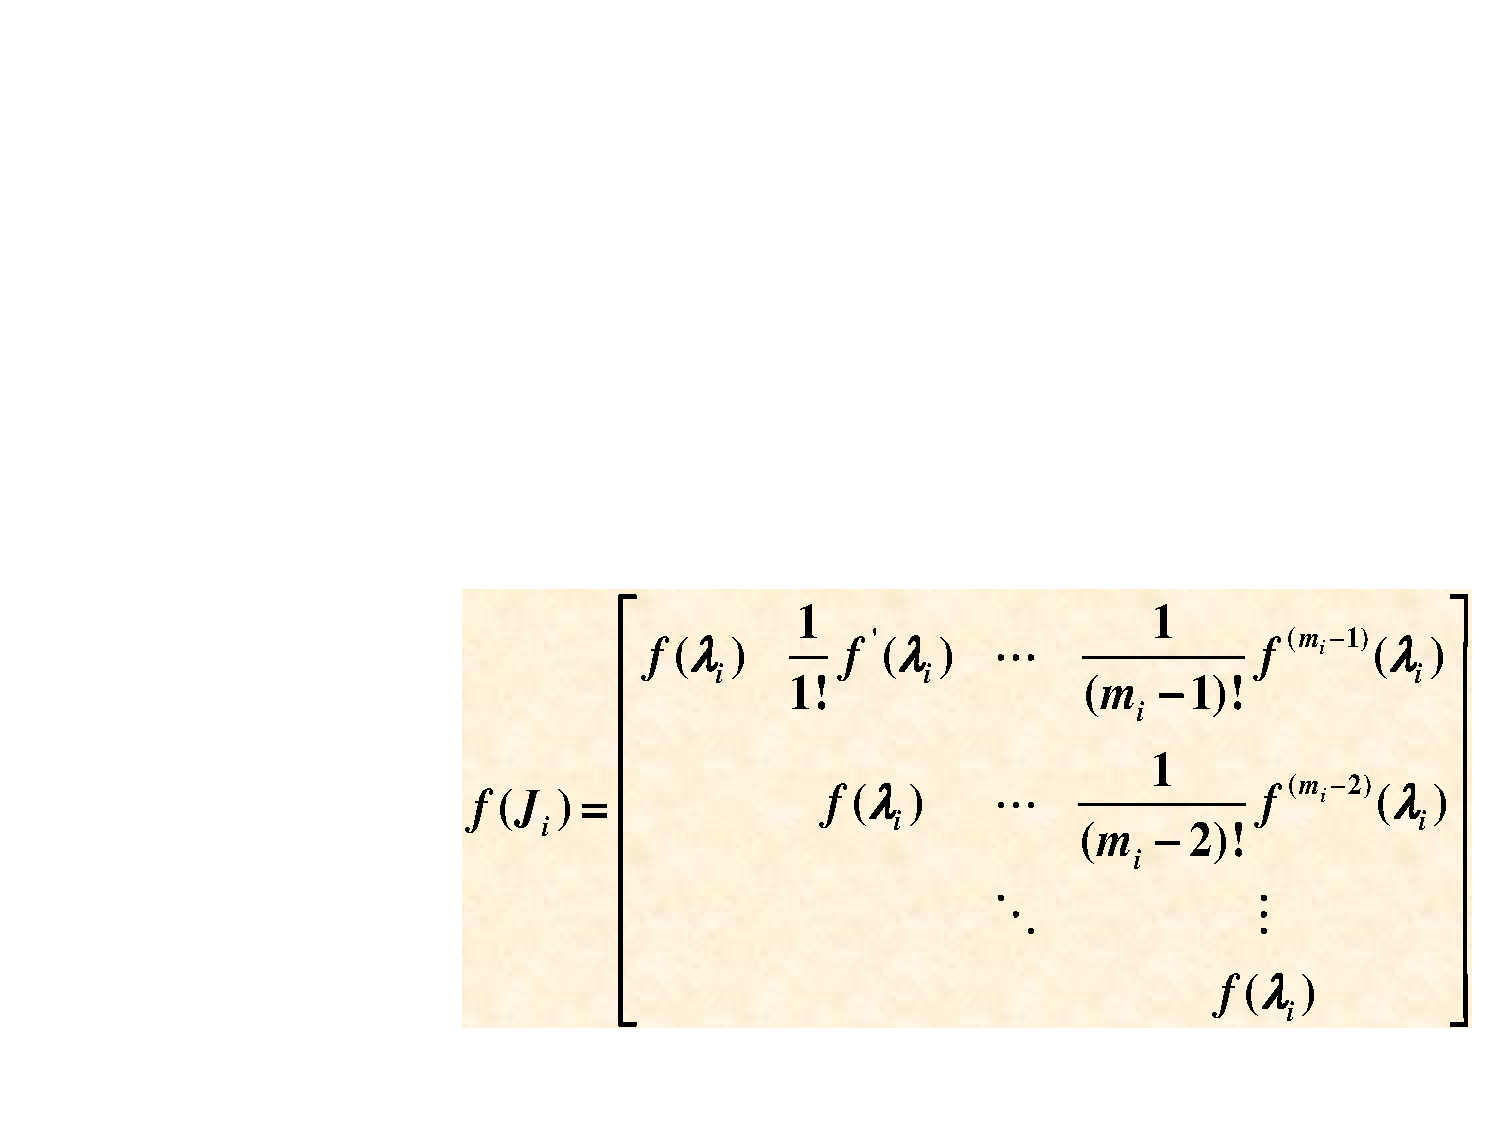
\includegraphics[scale=0.7]{image/52.pdf}  
	%\caption{信息包结构} 
	\label{fi}  
\end{figure}

\end{enumerate}

\subsubsection{矩阵函数的几种特殊情形}
\begin{enumerate}
	\item $A^2=A$
	
	$A^2=A(\lambda=0 \ or \ 1)\Rightarrow A^k=A$(\colorbox{yellow}{$k\geq 1$})
	
$\Rightarrow f(A)=\sum\limits_{k=0}^{\infty}c^kA^{k} =\sum\limits_{k=0}^{\infty}c_kA=c_0E+\sum\limits_{k=1}^{\infty}c_kA=c_0E+\sum\limits_{k=1}^{\infty}(c_k\cdot 1)A$

\colorbox{yellow}{$=c_0E+(f(1)-c_0)A$}
\begin{note}
	$e^A=E+(e-1)A\quad \sin A=(\sin1) A$
\end{note}
	
	\item $A^2=E$(对和矩阵)
	\[
	A^2=E\Rightarrow
	\left\{\begin{array}{l}
	A^{2k}=E\\
	A^{2k+1}=A 
	\end{array}\right.
	\Rightarrow f(A)=\sum\limits_{k=0}^{\infty}c_kA^{k}=\sum\limits_{k=0}^{\infty}c_{2k}E+\sum\limits_{k=0}^{\infty}c_{2k+1}A
	\]
	
\end{enumerate}
\begin{note}
	$\sin A=(\sin1) A \quad \cos A=\cos1$
\end{note}



